In this chapter we give an overview of the work (Par. \ref{overview}). We then present a taxonomy of the current state of the art (Par \ref{sota}) concerning computer vision lie detection. The last section is about the structure of this work and our contribution (Par \ref{contrib}).

\pagebreak

\section{Overview of the work} \label{overview}
fill

\pagebreak

\section{People Lie Detection} \label{pplLieDet}
most untrained people are no better than chance at detecting lies \cite{Porter2012SecretsAL}
People lie twice a day on average \cite{LyingEverydayLife}
lying frequency \cite{DigitalDeception} increased with online comunication
People often underestimate the effort they should take to spot liars, but have too much confidence on their judgment\cite{VrijDLD}
emotionally intelligent people perform worse at deception detection. This is due to their greater sympathetic feelings to others \cite{EmotionallyIntelligent}
In \cite{BondDePauloAccuracy} the authors analyze the accuracy of deception judgments from a collection of 206 documents and 24.483 judges. They found that people can differentiate lies and truths with an accuracy of 54\%, with a lie detection accuracy of 47\% and a truth detection accuracy of 61\%. Their findings reveal that is easier for people to discriminate lies from the audio cues rather than the visual ones. In another study \cite{HartwigGranhag} 192 students obtained an accuracy of 55.2\% on lie detection, with 61\% accuracy for guilty suspects and 49\% for innocent ones. Police officers and other trained officials seems to perform better at lie detection obtaining around 70\% accuracy at detecting both lies and truths correctly \cite{VrijPoliceDetect}.

% also talk about non-contact

\pagebreak

\section{State of the Art} \label{sota}
How are lies detected? At the moment there are a lot of different instruments and technologies to detect lies, ranging from the good old polygraph and cameras to MRI machines. 
In computer vision, lie detection is done using an array of different techniques, employing not only RGB cameras but also physical sensors and thermal cameras, with machine learning techniques, and often combining many of them to achieve better results. 
We now proceed to describe the state of the art, based on the latest researches done in the field:
%\pagebreak

\subsection*{Speech}
Speech is one of the many methods that can be used to recognize if a person is lying, in fact the speech signal contains linguistic, expressive, organic and biological data. \cite{norena}\\
One of the most used indicator of lying in various studies has been the response latency \cite{EaseLying}, since inventing a lie requires additional cognitive load as opposed to remembering the truth. The authors also notice that habitual lying makes it easier, and conversely often telling the truth makes lying harder.\\
Another indicator of lying is the speech rate when it's different from the normal rate \cite{TemporalCues}. Other verbal cues like grammar usage and word frequency have been used and have achieved high accuracy in psychological researches \cite{PorterTruthLying}.\\
Speech analysis can reveal changes that affect behavior, such as stress, emotion, deception etc. by analyzing the pitch and the stress level. When a stressful situation arise, the hormonal levels of the body change, and this causes an increase in blood pressure and heart rate. This in turn affects the muscle in the respiratory system, and so speech is affected \cite{norena}. \\
In sound processing, the mel-frequency cepstrum (MFC) is a representation of the short-term power spectrum of a sound. Mel-frequency cepstral coefficients (MFCCs) are coefficients that collectively make up an MFC \cite{wiki:mfcc}. \\
In \cite{relidss} the authors created a new database by making 40 candidates try to decive them while telling truthful or deceptive statements for about one to two minutes. From this experiment they extracted MFCC and pitch and processed them through Matlab's Voice Box. After acquairing the data an SVM classifier was trained to classify new data, obtaining an accuracy of Lie and Truth detection from speech audio respectively 88.23\% and 84.52\%. \\
In \cite{Perez-Rosas:2015:DDU:2818346.2820758} \cite{Mihalcea:2013:ADD:2522848.2522888} Perez et al. utilize real life trial data to identify deception, achieving 60-75\% accuracy employing a model that extracts features from both linguistic and gesture modalities.
%\pagebreak
 
\subsection*{Eyes}
Using the eyes to detect lies is one of the most studied approaches as the eyes hold a lot of information \cite{FUKUDA2001239}. Moreover is possible to generate a non invasive approach while analyzing the eyes. Cognitive load, which is set to increase while lying, is one of the most significant factor. Important are also the blink rate, gaze aversion and pupil dilation.\\
In \cite{8125844} the authors utilize high speed cameras to record and analyze blink count and blink duration of 50 subjects while asking 10 control questions, to see if there is a variation in them while the subject is being questioned. The authors analyzed the resulting images frame by frame and based on the facial landmarks around the eye they recognized AU45, the action unit for blinking. The results show that both blink duration and count are increased while lying.\\
In another study, Leal and Vrij \cite{Leal2008} asked 13 liars and 13 truth tellers to lie or tell the truth in a target period, while having a baseline from two preceding periods. The eye blinks during the target and baseline periods and directly after the target period (target offset period) were recorded. Compared to the baseline periods, lying subjects show a decrease in eye blinks during the target period and an increase in eye blinks during the target offset period. This pattern resulted very different for truth tellers. \\
Singh et al. in \cite{7324092} show that while lying there is an increase in cognitive load and a significant decrease in eye blinks, directly followed by an increase as soon as the cognitive demand ceases, after telling the lie. A threshold is set by the authors for this study, either at 26 blinks/minute or it is calculated personally using the average blink rate from a blink detection algorithm. Blink detection is done with MATLAB using the HAAR Cascade algorithm. \\
Lim et al. study eye gaze \cite{Lim:2013:LTE:2535948.2535954} to investigate the relation with lie detection. The result supports the theory that cognitive load decreases the number of eye movements.\\
Bhaskaran et al. measure deception by the deviation from normal behavior \cite{5771407} at critical points during an investigative interrogation. For starters a dynamic Bayesian model of the eye movement is trained during a normal conversation with each of the 40 subjects of the experiment, then the remainder of the conversation is broken into pieces and each piece is tested against the normal behavior. The deviation from normality are observed during critical points in the interrogation and used to deduce the presence of deceit, obtaining an accuracy of 82.5\%. \\
In \cite{7165946} Proudfoot et al. using latent growth curve modeling, research how the pupil diameter changes over the course of an interaction with a deception detection system. The assumption is that anxiety changes the pupil diameter. The subjects are presented with crime-relevant target items (possibly incriminating) and non relevant items. The results indicate that the trends in the changes are indicative of deception during the interaction, regardless if incriminating items are shown. \\
%is this useful at all???
%Nurcin et al. \cite{NURCIN2017417} analyze the segmentation of pupil and iris radius in images taken from the MMU iris database. The assumption is that bigger pupils are lying ones and small pupils are neutral. The algorithm does the segmentation of iris and pupil radius, and then trains a neural network to classify high and low pupil to iris radius. All images from the MMU database were correctly classified.
%\pagebreak

\subsection*{Neuroscience}
EEG and fMRI have been recently employed for lie detection with good results.
EEG (Electroencephalogram) is a monitoring method that records brain activities based on its potential. 
In \cite{7440177}  Simbolon et al, use ERP (Event Related Potentials) to measure brain response directly from thought or perception. Among the numerous types of signals that constitute the ERP signal, P300 is the most critical for lie detection. Eleven males of age between 20 and 27 took part in the study. The gathered data were then divided into training and test sets to produce different models. The highest accuracy of 70.83\% was reached by a SVM classifier in detecting lying subjects.\\
In \cite{Lai2017} twenty people were subject to a card test using an EEG. The authors used the EEG to identify frequency bands and measure lying state based on spectral analysis, with the use of fuzzy reasoning, obtaining 89.5\% detection accuracy. \\
Arasteh et al. \cite{7511728} use empirical mode decomposition (EMD) to extract features from the EEG signal. A genetic algorithm was then utilized for the feature selection. The classification accuracy of guilty and innocent subjects was 92.73\%.

\subsection*{Head}
Noje et al. \cite{7367432} set up a study with ten subjects to observe the potential of head movements in lie detection. They built an application to detect head movement and position by performing a frame to frame analysis on a video stream. A correlation was made between head movement/position and the identification of lies. The results of the study are not concluding as this data can't be utilized without being incorporated with other modalities such as voice, gaze, words, expressions et cetera.

\subsection*{Facial Expression}

\begin{figure}[!]
	\centering
	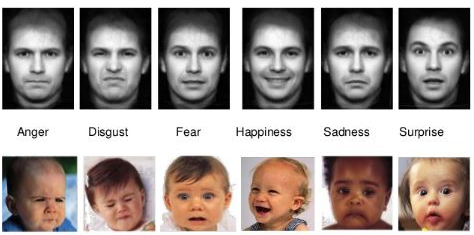
\includegraphics[width=3cm, height=4cm]{expr}
	\caption{Example of a parametric plot ($\sin (x), \cos(x), x$)}
\end{figure}

Facial micro-expressions are very fast (1/2 to 1/25 of a second) and involuntary expressions that come up on the human face when they are trying to suppress or hide an emotion. Micro-expressions have been used and classified since 1977 to recognize and distinguish real or fake emotions \cite{ekman}. \\
Substantial work on Micro-Expressions has been done by Pfister, Li et al. In \cite{pfister2011micro} they collect data with a high speed camera and use a temporal interpolation model to recognize micro expressions. In \cite{xli2012spontaneous} they unveil a new dataset, the Spontaneous Micro-expression Database (SMIC), which includes 164 microexpression video clips elicited from 16 participants. A study of spontaneous micro expression spotting and recognition methods is done in \cite{xli2015reading}. A new training free method, based on feature difference contrast, for recognizing micro-expressions is presented and revealed effective on unseen videos. A micro-expression framework is presented and tested on SMIC and CASMEII database with very good results. A new micro-expression analysis system (MESR) is presented and it is able to recognize micro-expressions from spontaneous video data. \\
Owayjan et al. \cite{6462897} designed a lie detection system using micro-expressions. At first an embedded video system is used to record the subject interview. The video stream is converted into frames, and each frame is processed in four stages: converting the images, filtering out useless features, applying geometric templates and finally extracting the measurements to detect the micro-expressions. Eight facial expressions can be recognized and lies can be discerned with high precision. \\
%maybe not exactly micro expr
In \cite{10.1007/978-3-319-47955-2_27} Kawulok et al. explore how to exploit fast smile intensity detectors to extract temporal features using a SVM classifier. Using exclusively a face detector, without localizing or tracking facial landmarks, they analyze the smile intensity time series. They then employ an SVM classifier to improve training from weakly labeled datasets. Then, to train the smile detectors, they use uniform local binary pattern features. This allows to detect, in real time, between spontaneous or posed expressions. \\
Su et al. \cite{SU201652} aim to test the validity of facial clues to deception detection in high-stakes situations using computer vision approaches. By using invariant 2D features from nine separate regions of the face they perform facial analysis on eye blink, eyebrow motion, wrinkle occurrence and mouth motion, integrated with a facial behavior pattern vector. Training a Random Forest to classify the patterns into deceptive or truthful, they achieved a 76.92\% accuracy.

\subsection*{Thermal}
In thermal imaging, thermal features are extracted from the face using a high definition thermal camera to analyze whether differences occur when a subject responded truthfully or deceptively. The most relevant zones are forehead and periorbital regions \cite{Rajoub} \cite{Abouelenien:2015:TAD:2823465.2823470}. \\
In \cite{6967765} data are gathered non-intrusively from the nostril and periorbital regions using two dimensional far infrared cameras. The temperature is converted in change in blood flow velocity and a signature of the respiration pattern is determined in terms of the ratio of the measured maximum and minimum temperatures in the nostril area. The classification rate for this study is 88.5\%.

\subsection*{Multimodal}
There are ways to detect lies that are a combination of different modalities. This improves the detection of deceptive behavior \cite{Abouelenien:2014:DDU:2663204.2663229}. \\
In \cite{Abouelenien:2016:ATV:2910674.2910682} Abouelenien et al. collect data from a dataset of 30 subjects to examine thermal and visual clues of deception. Their aim is to identify the regions that offer higher capability of detecting deceit. The method employed uses the CERT (Computer Expression Recognition Toolbox) to detect facial expression and encodes them with AU (Action Units). For thermal features they create a thermal map using grayscale and Hue Saturation Value. They also calculated normalized blinking rates and the mean head orientation angle along the entire length of the response. In addiction over 60 physiological features were extracted and stored. The experimental results show that the non-contact feature fusion model outperforms traditional physiological measurements, and that the forehead region is one of the most promising areas to gather information for deception detection.\\
In a following paper \cite{7782429} Abouelenien et al. explore a multimodal deception detection approach comprised of physiological, linguistic, and thermal features on a new dataset of 149 recordings. They determine the most discriminative region of the face based on thermal imaging, and perform feature analysis using a decision tree model. The result show that the forehead could be a better indicator of deceit than the periorbital area. The physiological features did not contribute very much, while the linguistic feature played a critical role, where self-referencing and exaggeration words where big indicators of deceit. The overall accuracy of the system is ~70\%\\
Another example of multimodal detection is found in \cite{DBLP:journals/corr/abs-1712-04415} where Wu et al. develop a framework to automatically detect deception in trials, while remaining hidden. They utilize three modalities: vision, audio and text. For vision, they employ various classifiers trained on low level video features to predict on human micro-expressions, to successively predict deception. Interestingly, IDT (Improved Dense Trajectory) features, often used to recognize actions in videos, are good predictors of deceptive behavior. The authors decided to fuse the score of the classifiers on IDT and micro-expressions to boost the performance. Regarding text, the transcript of the considered videos are analyzed, but the performance increase is very marginal. For speech, they integrate the vision side with MFCC features analysis from the audio, boosting the performances significantly, reaching an AUC of 0.877. \\

\pagebreak

\section{My Contributions} \label{contrib}


\section{Useful Things to Write and Cite}
Action Units \ref{au} \\
RNN LSTM \ref{lstm} \\

\subsection{Action Units} \label{au}
Substantial work on AU classification and intensity estimation has been done in \cite{Baltru2015} by Baltrusaitis et al. while developing the OpenFace \cite{Baltru2016} system. 


\pagebreak

\subsection{LSTM} \label{lstm}